

\actTitle{Worksheet 1.3}

\noindent
Student goals:
  \begin{itemize}
  \item Plot points in the coordinate plane.
  \item Identify the four quandrants of the coordinate plane.
  \item Calculate the distance between two points.
  \item Make rough sketch of the graph of a function by plotting
    points first.
  \item Determine the $x$ and $y$ intercepts of a function
    analytically and graphically.
  \end{itemize}


\noindent \textbf{Instructions:}  Work together in groups of  3 or 4 to complete the following problems.


\begin{enumerate}

\item Consider the relation that is defined by taking an object on your desk and assigning to it its color.  For example, if there is a hat on your desk that is green and blue, we would write
$$f(\text{hat}) = \{\text{green, blue}\}.$$
If there is a pen on your desk that is red, we would write
$$f(\text{pen}) = \text{red}.$$

\begin{enumerate}
\item List at least three items on your desk and come up with your own relation of this sort. (You can use imaginary items, if you need to.)
\vfil
\item What is the domain and range of your relation?
\vspace{.75in}
\item Is your relation a function?  Why or why not?
\end{enumerate}


\vspace{.5in}

\item Answer True or False.  In either case, verify your answer.

\begin{enumerate}
%\item $x=2$ is in the domain of $\displaystyle f(x)=\frac{x-2}{3x+1}$.
%\vfill
%\item $x=\frac{1}{3}$ is in the domain of $\displaystyle f(x)=\frac{x-2}{3x+1}$.
\item $x=-\frac{1}{3}$ is in the domain of $\displaystyle f(x)=\frac{x-2}{3x+1}$.
\vspace{.5in}
\item $x=-3$ is in the domain of $\displaystyle f(x)=\sqrt{x+3}$.
\vspace{.5in}
\item $x=-4$ is in the domain of $\displaystyle f(x)=\sqrt{x+3}$.
\end{enumerate}

\newpage


\item Determine the domain and range for each of the following functions.  Give your answer in interval notation.
\vspace{-.5in}
\begin{enumerate}

\item \ 
\begin{center}
	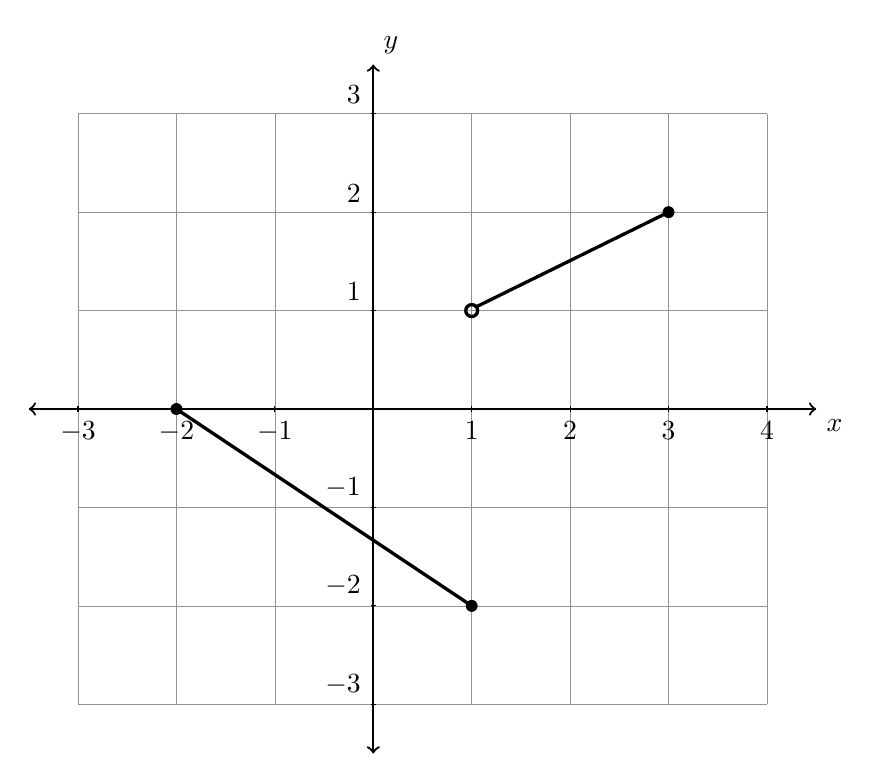
\begin{tikzpicture}[y=1.25cm, x=1.25cm,font=\sffamily,
  mydot/.style={
    circle,
    fill=white,
    draw,
    outer sep=0pt,
    inner sep=1.5pt
  }]
    %% Add a grid
    \draw[step = 1, gray, very thin,opacity=0.85] (-3, -3) grid ( 4, 3);
 	%% Draw the axes
	\draw[thick,<->] (-3.5,0) -- coordinate (x axis mid) (4.5,0) node[anchor = north west] {$x$};
    \draw[thick,<->] (0,-3.5) -- coordinate (y axis mid) (0,3.5) node[anchor = south west] {$y$};
    %% Label the y axis
    \foreach \y in {-3,-2,-1,1,2,...,3} {
      \draw (1pt, \y) -- (-1pt, \y) node[anchor = south east] {$\y$};
    }
    %% Label the x axis
    \foreach \x in {-3,...,-1,1,2,...,4} {
      \draw (\x,1pt) -- (\x,-1pt) node[anchor = north] {$\x$};
    }
    %% Draw the function.
    \begin{scope}
         \draw[scale=1.0,very thick,black] (-2, 0) -- (1,-2);
         \draw[scale=1.0,very thick,black] (1.05,1.04) -- (3,2);
         \fill[black] (-2, 0) circle[radius=0.5ex];
         \fill[black] (3,2) circle[radius=0.5ex];
         \fill[black] (1,-2) circle[radius=0.5ex];
         \draw[scale=1.0, very thick, black] (1,1) circle[radius=0.5ex];

    \end{scope}

    %%\node[above=0.1cm] at (-2,2 )   {\nextXValue};

  \end{tikzpicture}
\end{center}

\item \ 
\begin{center}
	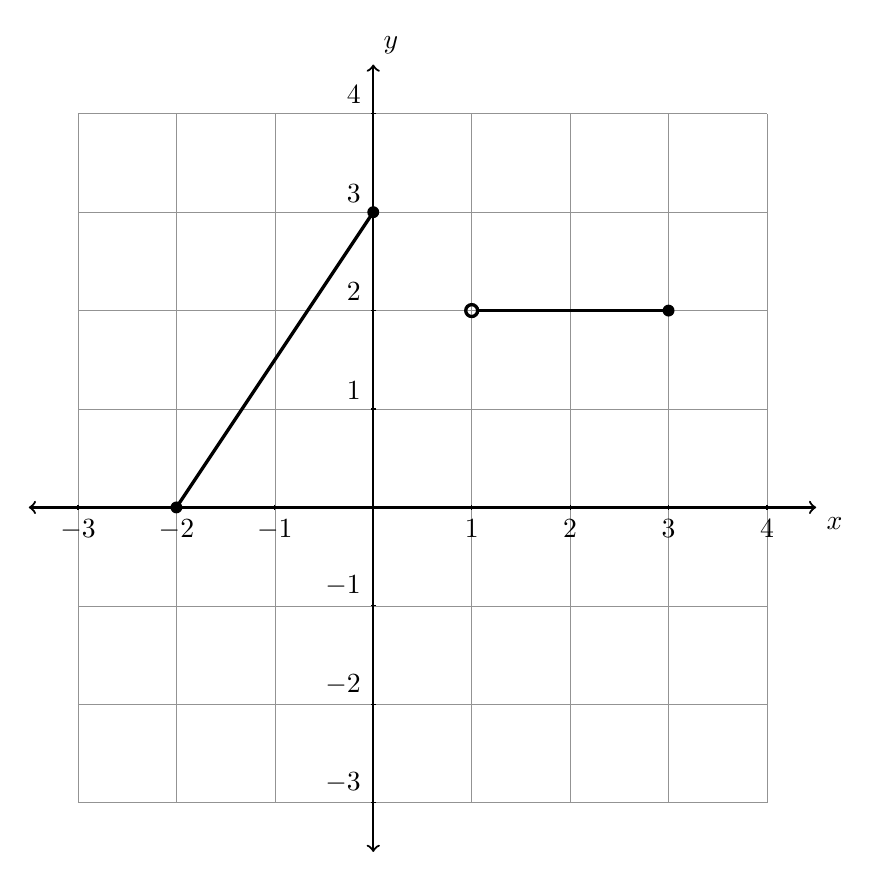
\begin{tikzpicture}[y=1.25cm, x=1.25cm,font=\sffamily,
  mydot/.style={
    circle,
    fill=white,
    draw,
    outer sep=0pt,
    inner sep=1.5pt
  }]
    %% Add a grid
    \draw[step = 1, gray, very thin,opacity=0.85] (-3, -3) grid ( 4, 4);
 	%% Draw the axes
	\draw[thick,<->] (-3.5,0) -- coordinate (x axis mid) (4.5,0) node[anchor = north west] {$x$};
    \draw[thick,<->] (0,-3.5) -- coordinate (y axis mid) (0,4.5) node[anchor = south west] {$y$};
    %% Label the y axis
    \foreach \y in {-3,-2,-1,1,2,...,3,4} {
      \draw (1pt, \y) -- (-1pt, \y) node[anchor = south east] {$\y$};
    }
    %% Label the x axis
    \foreach \x in {-3,...,-1,1,2,...,4} {
      \draw (\x,1pt) -- (\x,-1pt) node[anchor = north] {$\x$};
    }
    %% Draw the function.
    \begin{scope}
         \draw[scale=1.0,very thick,black] (-2, 0) -- (0,3);
         \draw[scale=1.0,very thick,black] (1.05,2) -- (3,2);
         \fill[black] (-2, 0) circle[radius=0.5ex];
         \fill[black] (3,2) circle[radius=0.5ex];
         \fill[black] (0,3) circle[radius=0.5ex];
         \draw[scale=1.0, very thick, black] (1,2) circle[radius=0.5ex];

    \end{scope}

    %%\node[above=0.1cm] at (-2,2 )   {\nextXValue};

  \end{tikzpicture}
\end{center}

\end{enumerate}

\newpage

\item Determine the domain of each of the following functions. Give your answer in interval notation.%\\[.5in]
\begin{enumerate}
\vspace{-.1in}
\item $g(x) = x^2$ \\[1in] 
\item $f(x)=\sqrt{3x-7}$ \vfill
%\item $f(x) = \dfrac{x+3}{x^2-9}$
\item $h(x)=\dfrac{5}{x^2-25}$ \vfill

\newpage
\item $f(x) = \sqrt{x^2-4x+3}$\vfill


\item $g(x) = \dfrac{\sqrt{x^2-4x+3}}{x^3+8}$\vfill

\end{enumerate}




\end{enumerate}














